%%%%%%%%%%%%%%%%%%%%% Reporte %%%%%%%%%%%%%%%%%%%%%
\documentclass[12pt, a4paper]{report}
\usepackage[spanish]{babel}
\usepackage[utf8]{inputenc}
%%%%%%%%%%%%%%%%%%%%% Paquetes %%%%%%%%%%%%%%%%%%%}		
\usepackage{geometry}
\usepackage{graphicx}
\usepackage{amssymb,amsmath,amsthm,amstext,amsfonts}
\usepackage{color}
%\usepackage{empheq}
%\usepackage{mdframed}
%\usepackage{booktabs}
%\usepackage{lipsum}
%\usepackage{psfrag}
%\usepackage{pgfplots}
%\usepackage{bm}
%\usepackage{multicol}
%\usepackage[T1]{fontenc}
%\usepackage[center, small]{caption2}
%\usepackage{array}
%\usepackage{textcomp}
%\usepackage{latexsym}
%\usepackage{titlesec}
%\usepackage[breakable]{tcolorbox}
%\usepackage{caption}
%\usepackage{float}
%\floatplacement{figure}{H} % forces figures to be placed at the correct location
%\usepackage{enumerate} % Needed for markdown enumerations to work
%\usepackage{fancyvrb} % verbatim replacement that allows latex
%\usepackage{grffile} % extends the file name processing of package graphics
%\usepackage[Export]{adjustbox} % Used to constrain images to a maximum size
%\adjustboxset{max size={0.9\linewidth}{0.9\paperheight}}
%\usepackage{titling}
%\usepackage{longtable} % longtable support required by pandoc >1.10
%\usepackage{calc}	   % table minipage width calculation for pandoc >= 2.11.1
%\usepackage{url}

\setlength{\parindent}{0pt}

\graphicspath{ {Img/} }

% Colors for the hyperref package
\definecolor{urlcolor}{rgb}{0,.145,.698}
\definecolor{linkcolor}{rgb}{.71,0.21,0.01}
\definecolor{citecolor}{rgb}{.12,.54,.11}

%%%%%%%%%%%% NEW THEOREM %%%%%%%%%%%%%%%%%
\providecommand{\abs}[1]{\lvert#1\rvert}
\newtheorem{definition}{Definición}
\newtheorem{proposition}{Proposición}
\newtheorem{remark}{Observación}
\newtheorem{notation}{Notación}
\newtheorem{lemma}{Lema}
\newtheorem{theorem}{Teorema}
\newtheorem{example}{Ejemplo}
%%%%%%%%%%%%%%%%%%%%%%%%%%%%%%%%%%%%%%%%%%%%%%%%%

\title{Notas - Tesis de posgrado.}
\author{Eduardo Ortiz Romero}

%%%%%%%%%%%%%%%%%%%%%%%%%%%%%%%%%%%%%%%%%%%%%%%

\begin{document}
\maketitle
\tableofcontents

\chapter*{Introcucción}

El teorema de Poincaré-Bendixson es un resultado 
fundamental en la teoría de sistemas dinámicos,
que establece condiciones bajo las cuales una trayectoria en 
un espacio de fase no diverge ni se
acerca indefinidamente a ninguna otra trayectoria, sino que 
se limita a un conjunto cerrado y
acotado. En este texto exploraremos este importante teorema.
Además, analizaremos algunos ejemplos concretos de sistemas 
dinámicos en los que se cumple
el teorema de Poincaré-Bendixson, así como situaciones en 
las que no se cumple.\\

\begin{figure}[h]
	\centering
	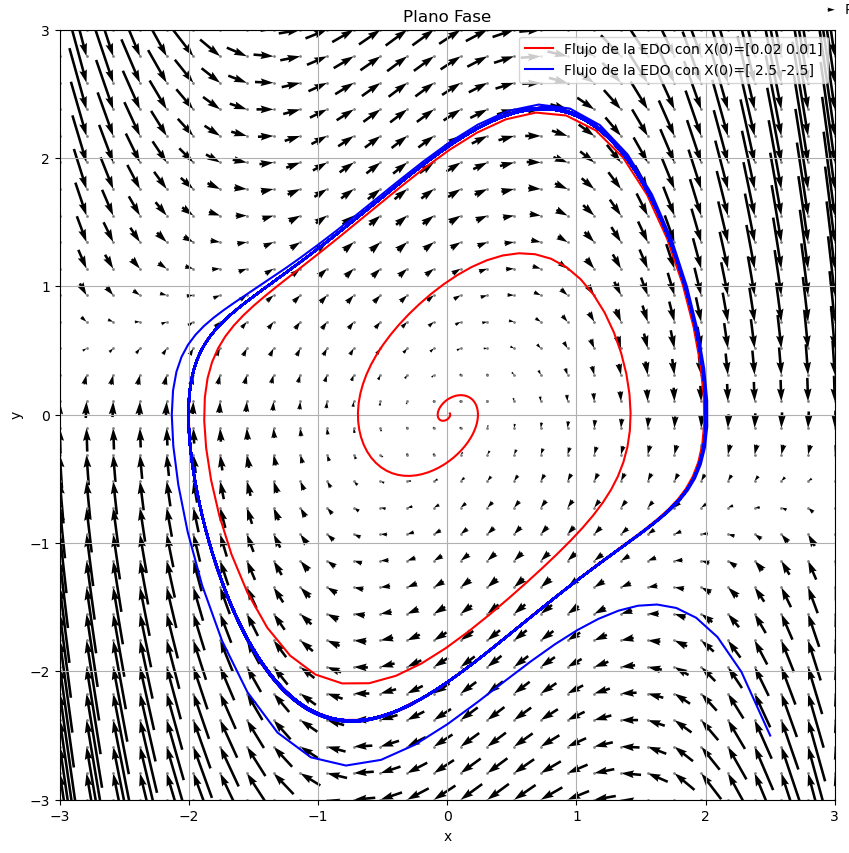
\includegraphics[width=8.5cm]{portada.png}
	\caption{Plano fase.}
\end{figure}

\newpage

\chapter{Preliminares}

\section{Coordenadas polares}

Dada la variable $(x,y)\in\mathbb{R}^2$ en el plano, 
definimos el cambio de coordenadas cartecianas $(x,y)$ 
a coordenadas polares $(r,\theta)$  con la relación:

\begin{equation}\label{eq: xpolar}
	x=r\cos(\theta)
\end{equation}

\begin{equation}\label{eq: ypolar}
	y=r\sin(\theta)
\end{equation}

Estas ecuaciones cumplen las siguientes identidades:

\begin{equation}\label{eq: r2}
	r^2=x^2+y^2\\
\end{equation}

\begin{equation}\label{eq: theta}
	\theta=\arctan{(\frac{y}{x})}
\end{equation}

Tenemos que $x=x(t)$ y $y=y(t)$, derivando a $\eqref{eq: r2}$ respecto de $t$
	      $$	2r\frac{dr}{dt}=2x\frac{dx}{dt}+2y\frac{dy}{dt} $$

se obtiene la ecuación equivalente:

\begin{equation}\label{eq: drcart}
		      rr'=xx'+yy'
\end{equation}

Derivando a $\eqref{eq: theta}$ respecto de $t$
	      $$\frac{d\theta}{dt}=\frac{1}{1+(\frac{y}{x})^2}(\frac{x\frac{dy}{dt}-y\frac{dx}{dt}}{x^2})=\frac{x\frac{dy}{dt}-y\frac{dx}{dt}}{x^2+y^2}$$

se obtiene la ecuación equivalente:
	      
\begin{equation}\label{eq: dthetacart}
		      r^2\theta'=xy'-yx'
\end{equation}


\chapter{Ciclos límite.}
\section{Motivación}

Consideremos el sistema no lineal

\begin{equation}\label{eq: sis1}
	\begin{matrix}
		x'=-y+x(1-x^2-y^2) \\
		y'=x+y(1-x^2-y^2)
	\end{matrix}
\end{equation}

con las condiciones iniciales $x(0)=x_0$, $y(0)=y_0$.\\

Para realizar un análisis cualitativo del sistema vamos a hacer un cambio
de coordenadas de cartecianas a polares, con el fin de simplificar
el sistema, después vamos a resolver cuantitativamente el  problema y
analizaremos algunas propiedades con ayuda de la solución analítica.\\

Con el cambio de coordenadas $\eqref{eq: xpolar}$ y  $\eqref{eq: ypolar}$ tenemos
las condiciones iniciales $r(0)=r_0$ y $\theta(0)=\theta_0$.\\

Sustituimos el sistema $\eqref{eq: sis1}$ en $\eqref{eq: drcart}$:
$$rr'=xx'+yy'=x[-y+x(1-x^2-y^2)]+y[x+y(1-x^2-y^2)]$$
$$rr'=x^2(1-x^2-y^2)+y^2(1-x^2-y^2)=(x^2+y^2)[1-(x^2+y^2)]$$
luego sustituimos $\eqref{eq: r2}$
$$rr'=r^2(1-r^2)$$
\begin{equation}\label{eq: drsis1}
	r'=r(1-r^2)
\end{equation}\\

Por otro lado sustituimos el sistema $\eqref{eq: sis1}$ en $\eqref{eq: dthetacart}$:
$$r^2\theta'=xx'-yy'=x[x+y(1-x^2-y^2)]-y[-y+x(1-x^2-y^2)]$$
$$r^2\theta'=x^2+y^2=r^2$$
\begin{equation}\label{eq: dthetasis1}
	\theta'=1
\end{equation}

Las ecuaciones $\eqref{eq: drsis1}$ y $\eqref{eq: dthetasis1}$ 
forman un sistema de ecuaciones no lineal desacoplado.\\

Comenzamos el análisis cualitativo de la ecuación diferencial $\eqref{eq: drsis1}$.\\

Sea $f(r)=r(1-r^2)$ con $r\geq0$, las soluciones de equilibrio son $r=0$ y $r=1$.
\begin{enumerate}
	\item Si $0<r<1$, entonces $r'=f(r)>0$, por lo tanto $r=0$ es un punto fuente o repulsivo.
	\item Si $1<r$, entonce $r'=f(r)<0$, por lo tanto $r=1$ es un sumidero o atractor.
\end{enumerate}\\

Las soluciones convergen a $r=1$.
\begin{figure}[h]
	\centering
	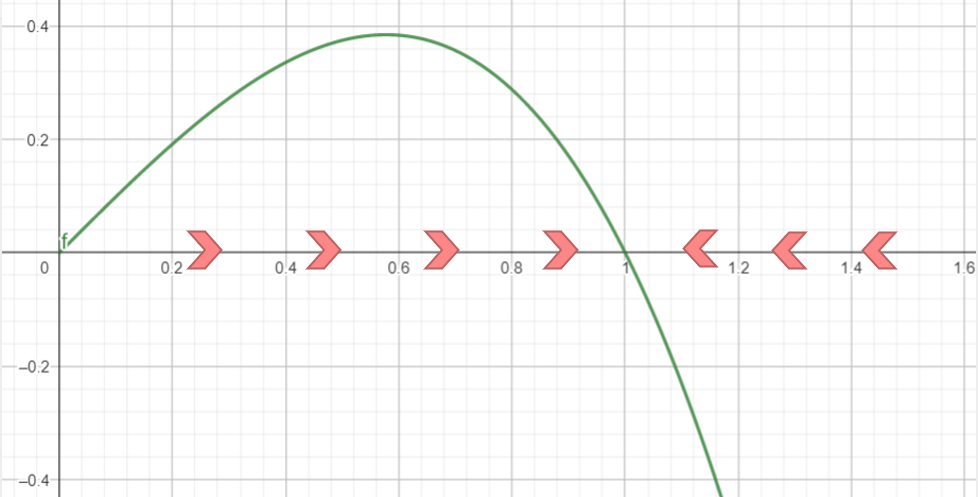
\includegraphics[width=14cm]{rej1.png}
	\caption{Plano fase de $\refeq{drsis1}$.}
\end{figure}\\

Por otro lado para $\eqref{eq: dthetasis1}$ la solución es $\theta(t)=t+\theta_0$,
donde $\theta_0=\theta(0)$.\\

Las soluciones del sistema $\eqref{eq: sis1}$ convergen a puntos sobre la
circunferencia centrada en el origen de radio $1$.\\

Resolvamos el problema de forma analítica.\\

La ecuación $\eqref{eq: drsis1}$ es separable
$$\int\frac{dr}{r(1-r^2)}=\int dt$$
integramos por fracciones parciales

$$\int\frac{dr}{r(1-r^2)}=\int\frac{dr}{r}-\int\frac{dr}{2(r+1)}-\int\frac{dr}{2(r-1)}$$
$$=\ln |r|-\frac{1}{2}\ln|r+1|-\frac{1}{2}\ln|r-1|+c_1$$

entonces
$$\ln |r|-\frac{1}{2}\ln|r+1|-\frac{1}{2}\ln|r-1|=t+c$$

desarrollamos logaritmos
$$\ln\left\lvert\frac{r^2}{r^2-1}\right\rvert=2t+c$$
$$\frac{r^2}{r^2-1}=ce^{2t}$$

$$r^2=\frac{e^{2t}}{c+e^{2t}}$$

Como $r\geq 0$
$$r=\frac{e^t}{\sqrt{c+e^{2t}}}$$
Aplicamos la condición inicial $r(0)=r_0$.\\
\\Las soluciones en coordenadas polares son:
\begin{equation}\label{eq: rsis1}
	r(t)=\frac{e^t}{\sqrt{\frac{1}{r_0^2}-1+e^{2t}}}
\end{equation}
\begin{equation}\label{eq: thetasis1}
	\theta(t)=t+\theta_0
\end{equation}
Dejaremos nuestra solución en coordenadas polares para realizar el siguiente
análisis del comportamiento asintótico.\\
\begin{enumerate}
	\item Si $r_0=1$ tenemos las ecuaciones
	      $$r(t)=1$$
	      $$\theta(t)=t+\theta_0$$
	\item Por otro lado, si $r_0>1$.
	      $$\lim_{t\to\infty}r(t)=\lim_{t\to\infty}\frac{e^t}{\sqrt{\frac{1}{r_0^2}-1+e^{2t}}}=1$$
	      $$\lim_{t\to-\infty}r(t)=\lim_{t\to-\infty}\frac{e^t}{\sqrt{\frac{1}{r_0^2}-1+e^{2t}}}=\infty$$
	\item Para $0<r_0<1$.
	      $$\lim_{t\to\infty}r(t)=\lim_{t\to\infty}\frac{e^t}{\sqrt{\frac{1}{r_0^2}-1+e^{2t}}}=1$$
	      $$\lim_{t\to-\infty}r(t)=\lim_{t\to-\infty}\frac{e^t}{\sqrt{\frac{1}{r_0^2}-1+e^{2t}}}=0$$
\end{enumerate}
Las trayectorias convergen a la circunferencia con centro en el origen
y de radio  $1$.\\

¿Qué significa que las trayectorias convergen a la circunferencia de centrada en el origen y de radio $1$?

\begin{definition} [Punto $\omega$ límite]
	Decimos que $\vec{z}\in\mathbb{R}^2$ es un punto $\omega$-límite
	de $\vec{x}_0\in\mathbb{R}^2$ si existe sucesión creciente de
	tiempos $\{t_n\}_{n\in\mathbb{N}}$
	con $t_n \to\infty$ cuando $n\to \infty$ tal que:
	$$\lim_{n\to\infty}\varphi^{t_n}(\vec{x}_0)=\vec{z}$$
\end{definition}

Regresemos las soluciones $\eqref{eq: rsis1}$ y $\eqref{eq: thetasis1}$ a
coordenadas cartesianas, con $\eqref{eq: xpolar}$ y $\eqref{eq: ypolar}$.
\begin{equation}\label{eq: xsis1}
	x(t)=\frac{e^t\cos(t+\theta_0)}{\sqrt{\frac{1}{r_0^2}-1+e^{2t}}}
\end{equation}
\begin{equation}\label{eq: ysis1}
	y(t)=\frac{e^t\sin(t+\theta_0)}{\sqrt{\frac{1}{r_0^2}-1+e^{2t}}}
\end{equation}

\begin{figure}[h]
	\centering
	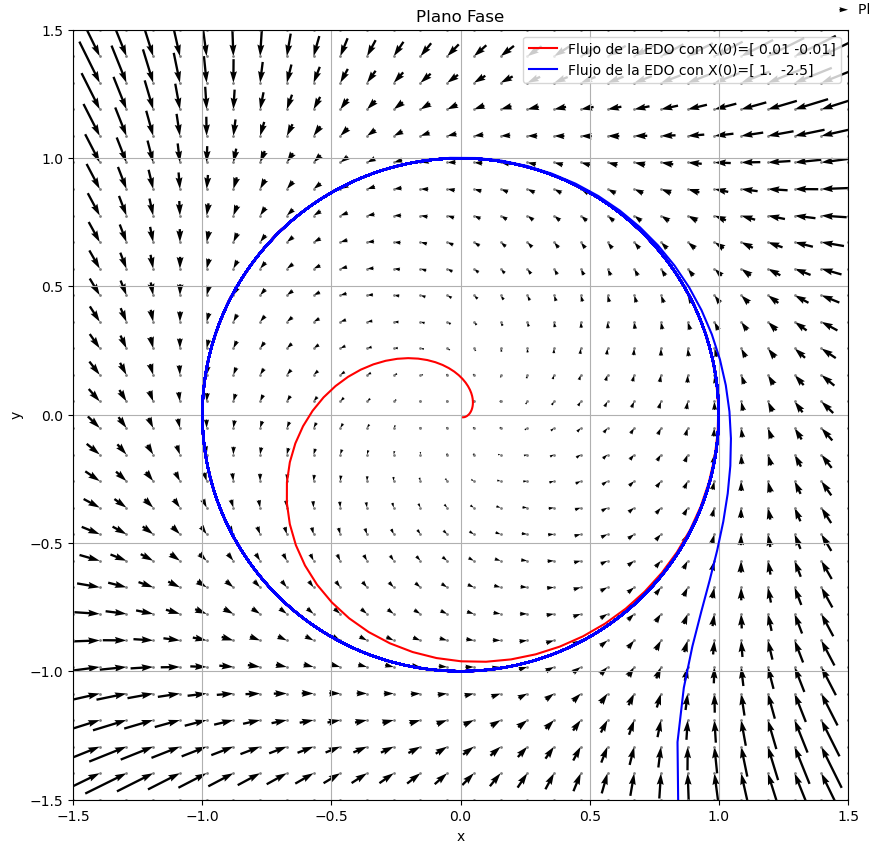
\includegraphics[width=13cm]{planofase1.png}
	\caption{Plano fase del sistema $\eqref{eq: sis1}$.}
\end{figure}

Tomemos la trayectoria en el plano fase de $\eqref{eq: sis1}$ que pasa por el punto
$(x_0,y_0)$, entonces existe $\theta_0=\arctan(\frac{y_0}{x_0})\in[0,2\pi]$.
La trayectoria que pasa por $(x_0,y_0)$ está dada por las ecuaciones $\eqref{eq: xsis1}$ y
$\eqref{eq: ysis1}$ donde $x_0=x(0)$ y $y_0=y(0)$.\\
\\Tomemos un punto en la circunferencia centrada en el origen con radio $1$,
supongamos que
en coordenadas polares tiene un álgulo $0<\alpha_0<2\pi$, veamos que es punto $\omega$ límite, para eso podemos definir
$\{t_n=2\pi n+\alpha_0-\theta_0\}_{n\in \mathbb{N}}$, entonces
$$\lim_{n\to\infty}x(t_n)=\cos(\alpha_0)$$
$$\lim_{n\to\infty}y(t_n)=\sin(\alpha_0)$$
en efecto el punto $(\cos(\alpha_0),\sin(\alpha_0))$ es un punto $\omega$ límite, esto
quiere decir que para cada punto de la circunferencia podemos encontrar
una sucesión de tiempos $\{t_n\}_{n\in \mathbb{N}}$ con $t_n\to\infty$ tal que la
trayectoria converge a ese punto de la circunferencia, es decir cualquier punto que se encuentra en la
circunferencia centrada en el origen y de radio $1$ es un punto $\omega$ límite de $(x_0,y_0)$,
entonces diremos que esta circunferencia es un conjunto $\omega$ límite de $(x_0,y_0)$, donde 
el conjunto $\omega$ límite se define como 

$$\omega(\vec{X}_0)=\{\vec{z}\in\mathbb{R}^2\mid\vec{z} \text{  es  } \omega\text{-límite de  } \vec{X}_0\}.$$

Además, notemos que para $\{t_n=2\pi n+\alpha_0-\theta_0\}_{n\in \mathbb{N}}$,
la sucesión $\{(x(t_n),y(t_n))\}_{n\in\mathbb{N}}$ es una sucesión
de puntos convergente tal que sus puntos son colineales sobre la recta
$L=\{(x,y)\in\mathbb{R}^2\mid y=\tan(\alpha_0)x \}$. Las intersecciones de las trayectorias
son los valores de la sucesión colineal.\\

Modifiquemos el sistema $\eqref{eq: drsis1}$, a un sistema perturbado
con $0\leq\epsilon<1$.
\begin{equation}\label{eq: drmod}
	r'=r(1-r^2)+\epsilon r\cos(\theta)
\end{equation}
Veamos si existe $r_{max}$ tal que $r'<0$ y $r_{min}$ tal que $r'>0$.\\

Reescribimos $\eqref{eq: drmod}$ como $r'=r(1-r^2+\epsilon \cos(\theta))$, como $r>0$,
entonces el signo de $r'$ depende de $1-r^2+\epsilon \cos(\theta)$.
Tenemos los siguientes casos:

\begin{enumerate}
	\item Si $1-r^2+\epsilon\cos(\theta)\leq 1-r^2+\epsilon<0$
	      entonces $\sqrt{1+\epsilon}<r_{max}$, por lo que para $r<r_{max}$ se tiene que $r'<0$.
	\item Por otro lado, si	$1-r^2+\epsilon\cos(\theta)>1-r^2-\epsilon>0$
	      entonces $\sqrt{1-\epsilon}>r_{min}$, por lo que para $r>r_{min}$ se tiene que $r'>0$.
\end{enumerate}

Las trayectorias que pasan por puntos en la circunferencia centrada
en el origen y con radio $r_{min}$
divergen del exterior de dicha circunferencia. Por otro lado,
las trayectorias que pasan por puntos en la circunferencia centrada
en el origen con radio $r_{max}$
convergen al interior del círculo.
A este segmento del plano lo llamamos región de atrapamiento.\\
\\Podemos intuir que debe existir
una curva cerrada en el interior, donde $r_{min}<r<r_{max}$, en la cual
las trayectorias convergen o alcanzan el equilibrio, de manera similar
a lo observado en el ejemplo
inicial, debido a su comportamiento. La idea de la existencia de una
curva cerrada de este tipo es lo que conocemos como ciclo límite.
\begin{figure}[h]
	\centering
	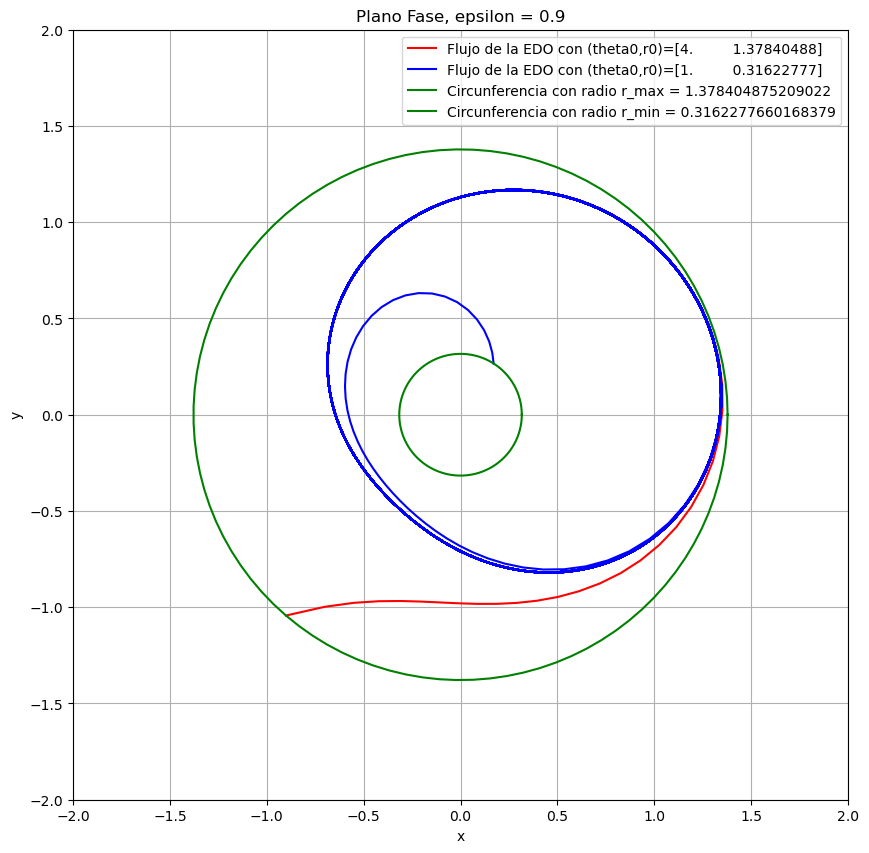
\includegraphics[width=13cm]{rminrmax.png}
	\caption{Plano fase del sistema con perturbación.}
\end{figure}

\newpage

\begin{definition}
	Definimos
	$$\varGamma_{\vec{x}}^{+}=\{\vec{y}=\varphi(t,\vec{x})\mid t>0\}$$
	$$\varGamma_{\vec{x}}^{-}=\{\vec{y}=\varphi(t,\vec{x})\mid t<0\}$$
	$$\varGamma_{\vec{x}}=\varGamma_{\vec{x}}^{+}\cup\varGamma_{\vec{x}}^{-}$$
\end{definition}

\begin{definition}
	Decimos que un conjunto $U$ es positivamente invariante si dado $\vec{x}\in U$ entonces  $\varGamma_{\vec{x}}^{+}\subset U$
\end{definition}

\begin{definition}
	Decimos que un conjunto $U$ es negativamente invariante si dado $\vec{x}\in U$ entonces  $\varGamma_{\vec{x}}^{-}\subset U$
\end{definition}

Notemos que esta sección del plano donde $r_{min}<r<r_{max}$ es positivamente invariante.
\newpage

\section{Propiedades de $\omega$ y $\alpha$ límite.}

Veamos más propiedades de los puntos y el conjunto $\omega$ límite. Comenzamos definiendo su análogo,
que estudia su comportmiento asintótico para $t\to-\infty$.\\

\begin{definition}
	Decimos que $\vec{z}\in\mathbb{R}^2$ es un punto $\alpha$-límite
	de $\vec{X}_0\in\mathbb{R}^2$ si existe sucesión decreciente de
	tiempos $\{t_n\}_{n\in\mathbb{N}}$
	con $t_n \to-\infty$ cuando $n\to \infty$ tal que:
	$$\lim_{n\to\infty}\varphi^{t_n}(\vec{X}_0)=\vec{z}$$
\end{definition}


\begin{definition}
	Definimos el conjunto $\alpha$-límite como $$\alpha(\vec{x})=\{\vec{y}\in\mathbb{R}^2\mid\vec{y}
		\text{ es } \alpha\text{-límite de }\vec{x}\}\equiv\text{Conjunto }\alpha\text{-límite}$$
	donde
	$$\vec{y}=\lim_{t_i\to-\infty}\varphi(t_i,\vec{x})$$
	con $\{t_i\}_{i=1}^{\infty}$ sucesión decreciente a $-\infty$.
\end{definition}

Algunas propiedades
\begin{itemize}
	\item $\omega(\vec{x})=\omega(\varGamma_{\vec{x}}^{+})$
	      y $\alpha(\vec{x})=\alpha(\varGamma_{\vec{x}}^{-})$.\\
	\item Si $\vec{x}*$ es equilibrio de $\vec{x}'=f(\vec{x})$ entonces:
	      $$\omega(\vec{x}*)=\alpha(\vec{x}*)=\{\vec{x}*\}$$
	\item Si $\varGamma_0$ es una órbita periódica para un sistema $\vec{X}'=f(\vec{X})$, entonces
	      $$\omega(\varGamma_0)=\alpha(\varGamma_0)=\varGamma_0$$.
\end{itemize}

\begin{lemma}
	Sea $\vec{x}\in\mathbb{R}^n$ tal que $\Gamma_{\vec{x}}^+$ esta acotada.
	Entonces:
	\begin{enumerate}
		\item $\omega(\vec{x})\neq\emptyset$
		\item $\omega(\vec{x})$ es acotado.
		\item $\omega(\vec{x})$ es cerrado.
		\item $\omega(\vec{x})$ es conexo.
	\end{enumerate}
\end{lemma}

\begin{lemma}
	Sea $\vec{x}\in\mathbb{R}^n$ con $\Gamma_{\vec{x}}^+$ acotada.
	Entonces
	$$\rho(\phi(t,\vec{x}),\omega(\vec{x}))\to0$$
	cuando $t \to \infty$.
\end{lemma}

\begin{lemma}[Invarianza]
	Sea $\Gamma_{\vec{x}}^+$ acotada. Entonces $\omega(\vec{x})$
	es invariante bajo el flujo
	$\varphi^t$, es decir, para cada $\vec{y}\in\omega(\vec{x})$ entonces
	$\varphi ^t(\vec{y})\in\omega(\vec{x})$.
\end{lemma}

\begin{lemma}
	Si $\omega(x)\neq\emptyset$ y no contiene puntos de equilibrio. Entonces contiene una órbita periódica $\varGamma_0$.
\end{lemma}

\begin{lemma}
	Si $\omega(x)$ contiene una órbita periódica $\varGamma_0$. Entonces $\omega(x)=\varGamma_0$.
\end{lemma}

\begin{theorem}[Poincaré-Bendixson]\label{TPB}
	Sea $\vec{x}\in\mathbb{R}^2$ tal que $\varGamma_{\vec{x}}^2\subseteq D\subseteq\mathbb{R}^2$ con $D\equiv$ Cerrado y acotado, 
	y conteniendo un número finito de equilirios de la EDO:
	\begin{equation}
		\begin{matrix}
			x' = f(x,y) \\
			y' = g(x,y)
		\end{matrix}
	\end{equation}
	entonces se cumple alguna de las siguientes:
	\begin{enumerate}
		\item $\omega(\vec{x})=\omega(\varGamma_{\vec{x}}^+)$ esta formado por un equilibrio.
		\item $\omega(\vec{x})$ es una órbita periódica.
		\item $\omega(\vec{x})$ está formada por equilibrios y órbitas que tienen a dichos equilibrios como puntos 
		$\alpha$ u $\omega$ límite.
	\end{enumerate}
\end{theorem}

\begin{definition}[Ciclo límite.]
	Decimos que la órbita periódica $\varGamma_0=\omega(\vec{x})$ 
	del caso $2$ del teorema $\ref{TPB}$ se llama
	\textbf{cliclo límite} si hay un anillo abierto que lo 
	ontenga y no hay otra órbita periódica en él, es decir 
	un ciclo límite es una órbita periódica aislada. 
	
\end{definition}

\begin{definition}
	La órbita que conecta a un punto silla consigo mismo (la intersección de la variedad estable con la inestable), se le llama curva homoclínica.
\end{definition}

\begin{definition}
	La órbita que conecta dos diferentes puntos de equilibrio se le llama curva heteroclínica.
	
\end{definition}
\newpage

\section{Teoría de promediación}

Como vimos determinar la existencia y propiedades cualitativas y cuantitativas 
de los ciclos límite en sistemas no lineales no es tarea fácil. En muchos 
casos los métodos analíticos fallan o se vuelve sumamente complejo y los 
métodos numéricos pueden ser ineficientes o inexactos. \\

El Método de Promediación es una herramienta poderosa y efectiva, 
parte de la teoría de perturbaciones y nos ayuda a simplificar el análisis 
de sistemas no lineales  transformando las ecuaciones originales en un sistema 
más manejable. La premisa fundamental es que, bajo ciertas condiciones, el 
comportamiento promedio del sistema a lo largo del tiempo puede revelar 
la existencia y la estructura de los ciclos límite.\\

La aplicación del Método de Premediación para verificar la existencia de 
ciclos límite en sistemas no lineales no solo proporciona una técnica 
analítica robusta sino que también ofrece una perspectiva más profunda 
del comportamiento oscilatorio inherente en dichos sistemas. Este enfoque 
no solo permite simplificar las ecuaciones diferenciales originales, sino 
también captar la esencia del comportamiento dinámico del sistema, 
facilitando así la identificación y caracterización de ciclos límite.\\

Definiendo el promedio local de una función y algunas de sus propiedades. 

\begin{definition}
	Sea $f:\mathbb{R}\times\mathbb{R}^p\to\mathbb{R}^n$ continua y $T>0$.
	Definimos:
	$$
		f_T(t,x)=\frac{1}{T}\int_{0}^{T}f(t+\tau,x)d\tau
	$$
	como el promedio local de $f$.
\end{definition}
\\
La función $f_T(t,x)$ calcula el valor promedio de la 
función $f(t,x)$ respecto a la variable $t$ en el intervalo $[t,t+T]$. 
Visto de otro modo, calcula del comportamiento promedio futuro, de $t$ a $t+T$. 
Es claro que si la función es $T$ periódica entonces $f_T(t,x)$ es constante $\forall t$.

\begin{proposition}
	Sea $f:\mathbb{R}\times\mathbb{R}^p\to\mathbb{R}^n$ continua y de periodo $T$ en $t$, entonces
	$$
		f_T(t,x)=f_0(x)
	$$
\end{proposition}
\\
Si la función a promediar es de Lipschitz entonces la diferencia entre ambas 
funciones está acotada, esto nos dice que el mapeo del promedio no se aleja demasiado 
de la función original, solo lo simplifica y guarda el comportamiento promedio
 de la función. 
\begin{proposition}
	Si $\phi:\mathbb{R}\to\mathbb{R}$ es de Lipschitz en $\mathbb{R}$, entonces
	$$
		\abs{\phi(x)-\phi_T(x)}\leq\frac{\lambda T}{2}
	$$
	i.e. $\phi(t)$ es $o(T)$ con respecto a $\phi_T(x)$.
\end{proposition}
\\
\begin{example}
	Consideremos la función $\phi(t)=\sqrt{t^2+1}$, esta función es de Lipschitz
	con constante $\lambda=1$, calculamos su promedio local con $T=0.5$

	$$\phi_T(t)=\frac{1}{2T}(((T + t)\sqrt{1 + (T + t)^2} + \sinh^{-1}(T + t)) - (t\sqrt{1 + t^2} + \sinh^{-1}(t)))$$

	graficamos ambas funciones. 

	\begin{figure}[h]
		\centering
		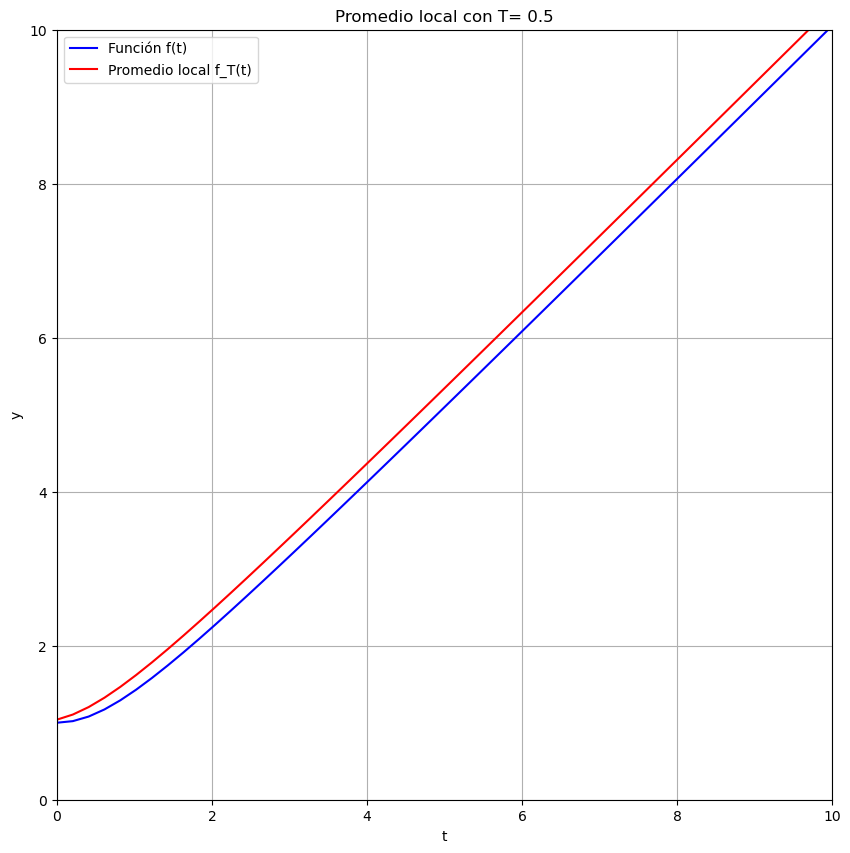
\includegraphics[width=10cm]{fl.png}
		\caption{Función vs  función promediada.}
	\end{figure}

la diferencia esta acotada por $M=\frac{\lambda T}{2}=\frac{0.5}{2}=0.25$. En este caso en la 
gráfica se puede observar que la diferencia converge a la cota $M$. 

\begin{figure}[h]
	\centering
	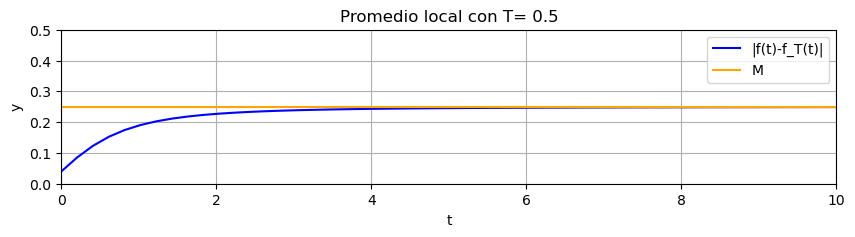
\includegraphics[width=13cm]{d.png}
	\caption{Diferencia de la Función con la función promediada.}
\end{figure}

\end{example}

\newpage


\begin{lemma}
	Consideremos la EDO
	$$
		x'=\epsilon f(t,x)
	$$
	con $x(0)=x_0$, donde $f$ es de Lipschitz en $x\in D\subseteq\mathbb{R}^n$
	y $f$ continua en $t\in[0,t]$.\\
	Sea $M=\sup_{x\in D} \sup_{0\leq\epsilon t\leqL} \abs{f(t,x)}<+\infty$
	\\Si $\phi(t)=\int_{0}^{t}f(\tau,x(\tau))d\tau$ con $x$ solución de la EDO.
	\\Entonces:
	$$
		\abs{\phi_T(t)-\int_{0}^{t}f_T(\tau,x(\tau))d\tau}\leq\frac{1}{2}(1+\lambda L)MT
	$$
	para $o(\frac{1}{\epsilon})=t$, donde $\lambda\equiv cte$ de Lipschitz.
	\\i.e. $\phi_T(t)=\int_{0}^{t}f_T(\tau,x(\tau))d\tau+o(T)$
\end{lemma}

\begin{lemma}
	Consideremos el problema de valor inicial
	$$
		x'=\epsilon f(t,x)
	$$
	$x(0)=x_0$, con $f$ Lipschitz en $x\in D\subseteq\mathbb{R}^n$ y continua
	en $t\in[0,t]$. \\
	Si $y$ es solución de $y'=\epsilon f_T(t,y)$, $y(0)=x_0$, entonces
	$$
		x(t)-y(t)=o(\epsilon T)
	$$
	p.t. $t=o(\frac{1}{\epsilon})$
\end{lemma}

\section{Oscilador de Van der Pol}
La ecuación del oscilador de Van der Pol describe el comportamiento de ciertos sistemas oscilantes no lineales.
Su fundamento físico se basa en el concepto de amortiguamiento no lineal y autodemostración de oscilaciones.
\begin{equation}\label{eq: VP}
	x''+x+\epsilon x'(x^2-1)=0
\end{equation}
donde $\epsilon$ es un parámetro de amortiguamiento no lineal.\\
\\El término $-\epsilon(1 - x^2)x'$ representa la no linealidad del amortiguamiento en el sistema. La expresión
$(1 - x^2)$ describe cómo el amortiguamiento varía en función de la posición del oscilador. Cuando $x$ es
pequeño, este término es cercano a $1$ y el amortiguamiento es lineal. Sin embargo, a medida que $x$
aumenta, el término $(1 - x^2)$ se hace más negativo, generando un efecto de amortiguamiento no lineal que
disminuye la velocidad del oscilador.\\
\\Extendemos a un sistema de ecuaciones.
\begin{equation}\label{eq: VPsis}
	\begin{matrix}
		y'=-x-\epsilon y(x^2-1) \\
		x'=y
	\end{matrix}
\end{equation}
Haremos el cambio de coordenadas a polares.
Sustituimos en $\eqref{eq: dxpolar}$ y $\eqref{eq: dypolar}$ en $\eqref{eq: VPsis}$
$$r\cos(\theta)\theta'+r'\sin(\theta)=-r\cos(\theta)-\epsilon r\sin(\theta)(r^2\cos^2(\theta)-1)$$
$$-r\sin(\theta)\theta'+r'\cos(\theta)=r\sin(theta)$$
entonces
\begin{equation}\label{eq: VPdr}
	r'=-\epsilon r\sin^2(\theta)(r^2\cos^2(\theta)-1)
\end{equation}
\begin{equation}\label{eq: VPdtheta}
	\theta'=-1-\epsilon r\sin(\theta)\cos(\theta)(r^2\cos(\theta^2)-1)
\end{equation}
Definimos para $\eqref{eq: VPdr}$ el promedio
\begin{equation}\label{eq: drbar}
	\bar{r}'=\bar{f}(\bar{r},\epsilon)
\end{equation}
donde
$$\bar{f}(\bar{r},\epsilon)=\frac{1}{2\pi}\int\limits_0^{2\pi}r'd\theta$$
Calculamos esta integral
$$\bar{f}(\bar{r},\epsilon)=\frac{1}{2\pi}\int\limits_0^{2\pi}-\epsilon r\sin^2(\theta)(r^2\cos^2(\theta)-1)d\theta$$
$$=\frac{1}{2\pi}[-\epsilon r^3\int\limits_0^{2\pi}\sin^2(\theta)\cos^2(\theta)d\theta+\epsilon r\int\limits_0^{2\pi}\sin^2(\theta)d\theta]$$
$$=\frac{1}{2\pi}[-\epsilon r^3[\frac{1}{32}(4\theta-\sin(4\theta))]_0^{2\pi}+\epsilon r[\frac{1}{2}(\theta-\sin(\theta)\cos(\theta))]_0^{2\pi}]$$
$$=\frac{1}{2\pi}[\frac{-\epsilon r^3}{32}(8\pi)+\frac{\epsilon r}{2}(2\pi)]=\frac{1}{2\pi}[\frac{-\epsilon r^3}{4}\pi+\epsilon r\pi].$$
Entonces
$$\bar{f}(\bar{r},\epsilon)=\frac{\epsilon r}{2}-\frac{\epsilon r^3}{8}$$
Pormediamos $\theta$
$$\bar{\theta}=2\pi t$$
Vamos a analizar $\eqref{eq: drbar}$
\begin{equation}\label{eq: drvander}
	\bar{r}'=\frac{\epsilon}{8}r(4-r^2)
\end{equation}
\begin{figure}[h]
	\centering
	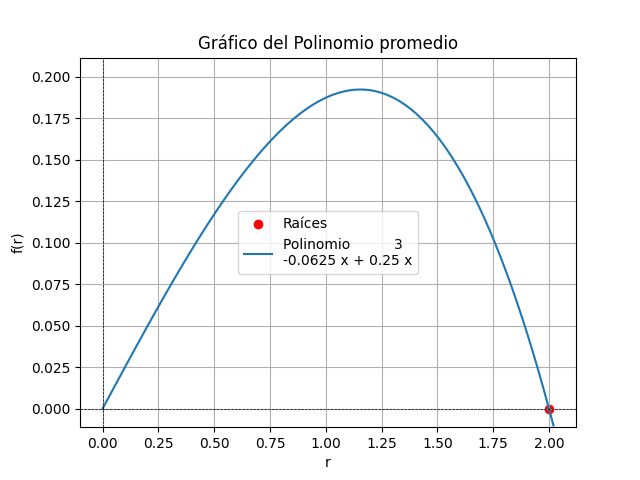
\includegraphics[width=12cm]{graficavanderpol.png}
	\caption{Plano fase de $\eqref{eq: drvander}$.}
\end{figure}
Las soluciones de equilibrio son $r=0$ y $r=2$.
\begin{enumerate}
	\item Si $0<r<2$, entonces $r'>0$, por lo que $0$ es un punto fuente o repulsivo.
	\item Si $r>2$, entonces $r'<0$, entonces $r=2$ es sumidero o atractor.
\end{enumerate}\\

\begin{figure}[h]
	\centering
	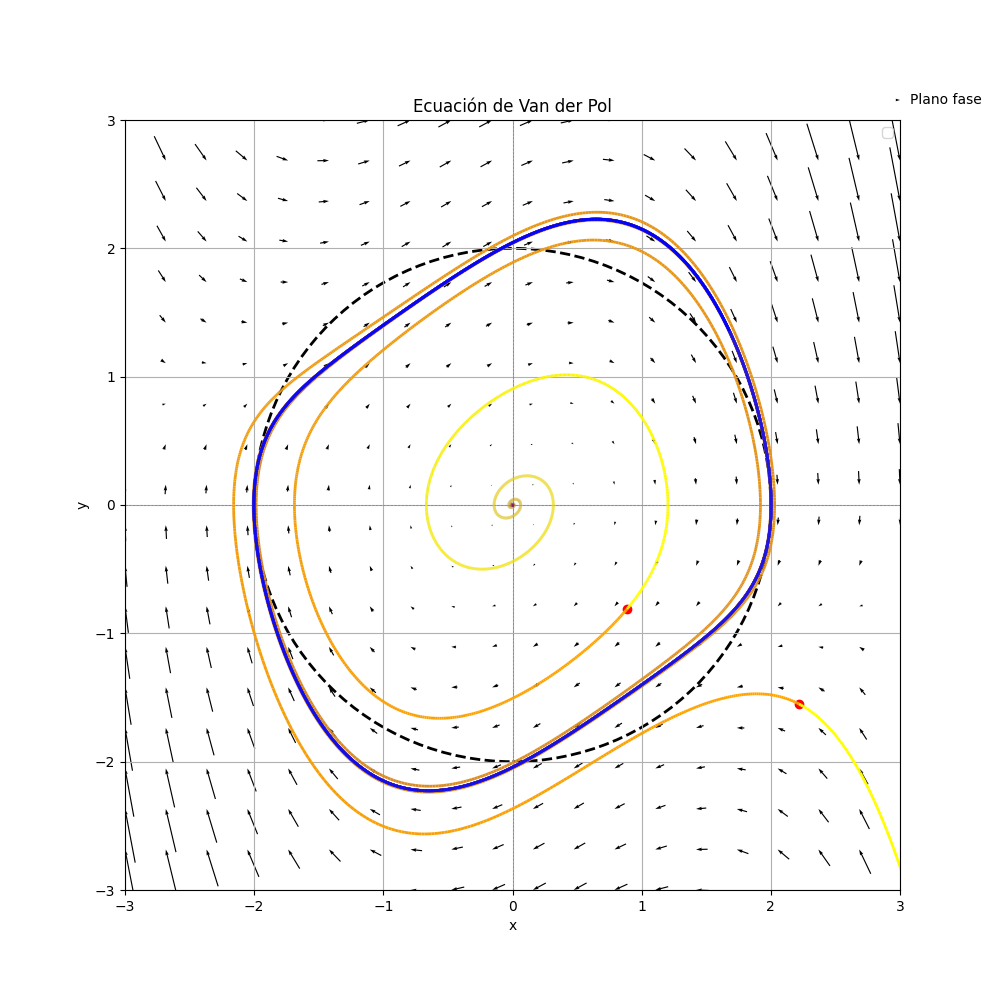
\includegraphics[width=11cm]{vanderpol.png}
	\caption{Plano fase. Dibujado en https://aeb019.hosted.uark.edu/pplane.html}
\end{figure}
\\Esto quiere decir que entre dos circunferencias de radios $0<r_{min}<2$ y $2<r_{max}$
existe al menos una curva cerrada a la cual las curvas convergen.

\newpage

\section{Ecuación de Rayleigh}
La ecuación de Rayleigh con amortiguamiento no lineal, se utiliza
para estudiar oscilaciones no lineales en sistemas mecánicos y se encuentra en
diversos campos como la mecánica estructural y la dinámica de sistemas físicos.

$$x''+\epsilon(x'^2-1)x'+x=0$$

El parámetro $\epsilon$ es un coeficiente que controla la influencia del término no lineal en el amortiguamiento.
El término $\epsilon(x'^2 - 1)x'$ es el término no lineal en el amortiguamiento. Mientras que en el amortiguamiento
lineal la fuerza de amortiguamiento es proporcional a la velocidad, en este caso el amortiguamiento depende de
la velocidad al cuadrado y se modifica por el término $(x'^2 - 1)$. Esto introduce un comportamiento no lineal en e
l sistema y puede dar lugar a fenómenos como la autoexcitación y la respuesta no armónica.
Extendemos a un sistema de ecuaciones.

\begin{equation}\label{eq: Rayleigh}
	\begin{matrix}
		y'=-\epsilon(y^2-1)y-x \\
		x'=y
	\end{matrix}
\end{equation}
Haremos el cambio de coordenadas a polares.
$$r\cos(\theta)\theta'+r'\sin(\theta)=-\epsilon (r^2\sin^2(\theta)-1)r\sin(\theta)-\omega^2r\cos(\theta) $$
$$-r\sin(\theta)\theta'+r'\cos(\theta)=r\sin(\theta)$$
Obtenemos la ecuación.
\begin{equation}\label{eq: Rayleighpolar}
	r'=\epsilon(1-r^2\sin^2(\theta))r\sin^2(\theta)+r\sin(\theta)\cos(\theta)(1-\omega^2)
\end{equation}
Definimos para $\eqref{eq: Rayleighpolar}$ el promedio
$$\bar{r}=\bar{f}(\bar{r},\epsilon)=\frac{1}{2\pi}\int\limits_0^{2\pi}r'd\theta$$
Calculamos esta integral
$$\bar{f}(\bar{r},\epsilon)=\frac{1}{2\pi}\int\limits_0^{2\pi}[\epsilon(1-r^2\sin^2(\theta))r\sin^2(\theta)+r\sin(\theta)\cos(\theta)(1-\omega^2)]d\theta$$
$$=\frac{1}{2\pi}\epsilon r\int\limits_0^{2\pi}\sin^2(\theta)d\theta-\frac{1}{2\pi}\epsilon r^3\int\limits_0^{2\pi}\sin^4(\theta)d\theta+\frac{1}{2\pi}r(1-\omega^2)\int\limits_0^{2\pi}\cos(\theta)\sin(\theta)d\theta$$
$$=\frac{1}{2\pi}\epsilon r[\frac{1}{2}(\theta-\sin(\theta)\cos(\theta))]\Big|_2^{2\pi}-\frac{1}{2\pi}\epsilon r^3[\frac{1}{32}(-8\sin(2\theta)+\sin(4\theta)+12\theta)]\Big|_0^{2\pi}+$$
$$\frac{1}{2\pi}r(1-\omega^2)[\cos^2(\theta)]\Big|_0^{2\pi}]=\frac{1}{2\pi}\epsilon r\pi-\frac{1}{2\pi}\epsilon r^3\frac{3}{4}\pi$$
$$=\frac{\epsilon r}{8}(4-3r^2)$$
Entonces tenemos el sistema
$$\bar{r}'=\frac{\epsilon r}{8}(4-3r^2)$$
$$\bar{\theta}'=2\pi t$$
Las soluciones de equilibrio son $r=0$ y $r=\frac{2}{3}\sqrt{3}$
\begin{figure}[h]
	\centering
	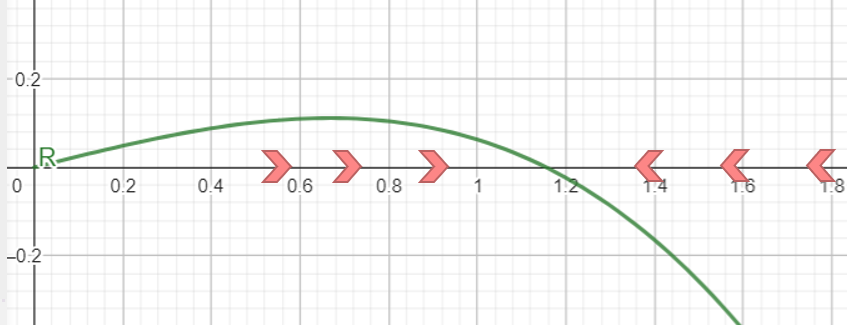
\includegraphics[width=9cm]{graficarayleigh.png}
	\caption{Plano fase.Dibujado en https://aeb019.hosted.uark.edu/pplane.html}
\end{figure}
\begin{figure}[h]
	\centering
	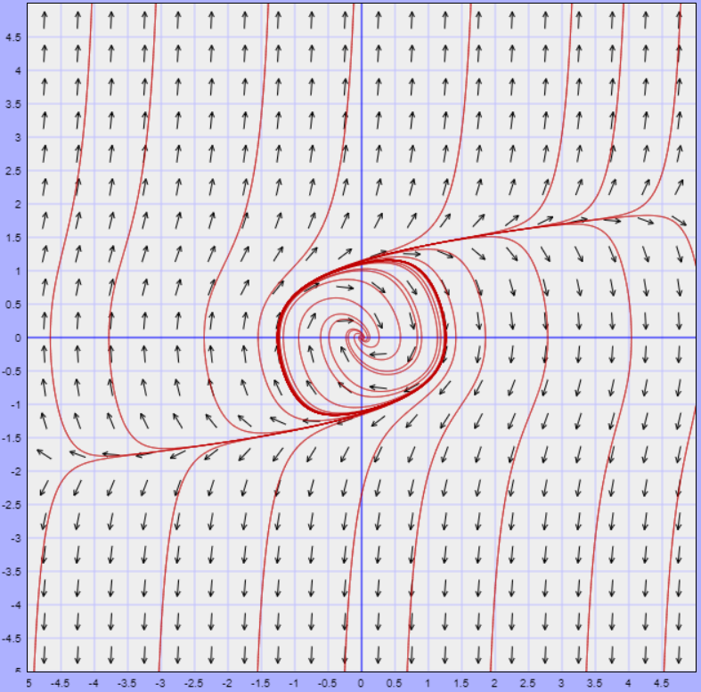
\includegraphics[width=11cm]{planorayleigh.png}
	\caption{Plano fase.Dibujado en https://aeb019.hosted.uark.edu/pplane.html}
\end{figure}

\newpage



\section{Sistemas Lienard}

Los sistemas Lienard son ecuaciones diferenciales de la forma:
\begin{equation}\label{eq: lienard}
	x''+f(x)x'+g(x)=0
\end{equation}
Para extender esta ecuacipon diferencial a un sistema de ecuaciones diferenciales. Primero definimos
$$F(x)=\int_0^xf(s)ds$$
entonces haciendo el cambio de variable $y=x'+F(x)$, obtenemos el sistema:
\begin{equation}\label{eq: lienardsystem}
	\begin{matrix}
		x'=y-F(x) \\
		y'=-g(x)
	\end{matrix}
\end{equation}
Vamos a enunciar el siguiente importante teorema.
\begin{theorem}[Lienard]
	Si $F(x)$ y $g(x)$ del sistema $\eqref{eq: lienardsystem}$ satisfacen las siguientes hipótesis:
	\begin{enumerate}
		\item $F,g\in C^1$.
		\item $F$ y $g$ son funciones impares.
		\item $xg(x)>0$ para todo $x\neq 0$.
		\item $F'(0)<0$
		\item $F$ tiene ceros sólo en $x=0$ o en $x=\pm a$.
		\item $F$ es monótona creciente en $(a,\infty)$ y $\lim_{x\to\infty}F(x)=\infty$
	\end{enumerate}
	entonces el sistema $\eqref{eq: lienardsystem}$ tiene un único ciclo límite y es estable.
\end{theorem}
Veamos que el sistema de ecuaciones asociado al Oscilador de Van der Pol es un sistema Lienard.
$$x''+\epsilon(x^2-1)x'+x=0$$
Definimos
$$F(x)=\int_0^x\epsilon(s^2-1)ds$$
$$=\epsilon[\frac{1}{3}s^3-s]| _0^x=\epsilon[\frac{1}{3}x^3-x]$$
Tenemos $F(x)=\frac{\epsilon}{3}[x^3-3x]$ y $g(x)=x$.\\
\\Podemos extender el oscilador de Van der Pol al sistema de ecuaciones:
$$
	\begin{matrix}
		x'=y-\frac{\epsilon}{3}[x^3-3x] \\
		y'=-x
	\end{matrix}
$$
Veamos si $F$ y $g$ satisfacen las hipótesis del teorema de Lienard
\begin{enumerate}
	\item En efecto $F,g\inC^1$.
	\item Notemos que las funciones son impares
	      $$F(-x)=\frac{\epsilon}{3}[(-x)^3-3(-x)]=\frac{\epsilon}{3}[-x^3+3x]=-\frac{\epsilon}{3}[x^3-3x]=-F(x)$$
	      $$g(-x)=-x=-g(x)$$.
	\item $xg(x)=x(x)=x^2>0$ para todo $x\neq 0$.
	\item $F'(0)=\epsilon(0^2-1)=-\epsilon<0$
	\item $F(x)=\frac{\epsilon}{3}[x^3-3x]=0$ entonces $F$ tiene raíces en $x=0$ y  $x=\pm \sqrt{3}$
	\item Si $y>x>\sqrt{3}$, entonces $y^3-3y>x^3-3x$, por lo que $F$ es monótona creciente. Además
	      por ser una función polinomial se tiene que
	      $$\lim_{x\to\infty}F(x)=\infty.$$
\end{enumerate}
Por lo tanto, por el teorema de Lienard el oscilador de Van der Pol tiene un único ciclo límite y es estable.
Esto ya lo comprobamos anteriormente, pero este teorema nos garantiza que es el único ciclo límite.

\section{Van der Pol y Rayleigh}
Ahora vamos a analizar la EDO
\begin{equation}\label{eq: vdpr}
	x''+\epsilon(x'^2-1)x'+\eta(x^2-1)x'+x=0
\end{equation}
Extendemos esta ecuación a un sistema de ecuaciones haciendo el
cambio de variable usual $y=x'$. Obetenemos lo siguiente:
\begin{equation}\label{eq: vpdrsis}
	\begin{matrix}
		y'=-\epsilon(y^2-1)x'-\eta(x^2-1)y-x \\
		x'=y
	\end{matrix}
\end{equation}
Hamos un cambio de coordenadas a polares. Sustituimos $\eqref{eq: dxpolar}$ y
$\eqref{eq: dypolar}$ en nuestro sistema, obtenemos:
$$r'\sin(\theta)+\theta'r\cos(\theta)=-\epsilon(r^2\sin^2(\theta)-1)r\sin(\theta)-\eta(r^2\cos^2(\theta)-1)r\sin(\theta)-r\cos(\theta)$$
$$r'\cos(\theta)-\theta'r\sin(\theta)=r\sin(\theta)$$
Calculamos $r'$ y $\theta'$
\begin{equation}\label{eq: drvdpr}
	r'=-[\epsilon(r^2\sin^2(\theta)-1)+\eta(r^2\cos^2(\theta)-1)]r\sin^2(\theta)
\end{equation}
$$\theta'=-[\epsilon(r^2\sin^2(\theta)-1)+\eta(r^2\cos^2(\theta)-1)]\cos(\theta)\sin(\theta)-r$$
Vamos a promediar $r'$, calculamos $\bar{r}'$:
$$\bar{r}'=\frac{1}{2\pi}\int_0^{2\pi}-[\epsilon(r^2\sin^2(\theta)-1)+\eta(r^2\cos^2(\theta)-1)]r\sin^2(\theta)d\theta$$
$$=-\frac{r^3}{8}(3\epsilon+\eta)+\frac{r}{2}(\epsilon+\eta)$$
Calculamos las raíces no negativas de $\bar{r}'=-r^3(\frac{3\epsilon+\eta}{8})+r(\frac{\epsilon+\eta}{2})$, estas son
$r_1=0$ y $r_2=2\sqrt{\frac{\epsilon+\eta}{3\epsilon+\eta}}$.\\
\\Para los valores de $\epsilon=0.5$ y $\eta=0.4$ el valor de el atractor es $r_2=1.3764\dots$, podemos ver en la imagen que en efecto
existe un ciclo límite aproximado a la circunferencia de radio $r_2$.

\begin{figure}[h]
	\centering
	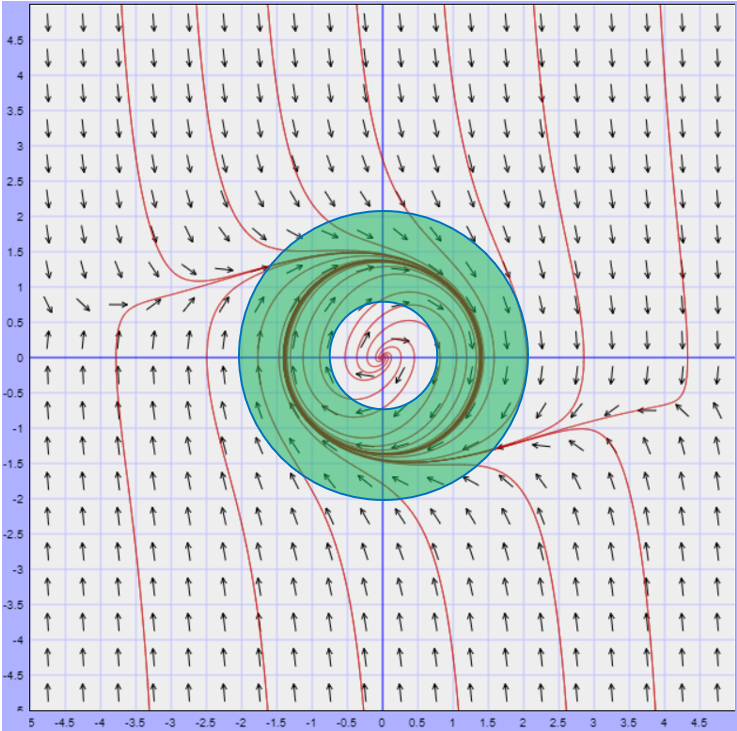
\includegraphics[width=9cm]{VDP-R.png}
	\caption{Plano fase.Dibujado en https://aeb019.hosted.uark.edu/pplane.html}
\end{figure}

\newpage








\end{document}
